\documentclass{beamer}

\usetheme{Antibes}
\usepackage{pgfplots}
\title[Prasaanth&Varun]{Solving 2D geometry using MATRICES}
\subtitle{Matrix Project}
\author{Prasaanth-EE18BTECH11032\\Varun-EE18BTECH11030}


\begin{document}

\begin{frame}
\titlepage    
\end{frame}

\section{Question}
\begin{frame}{Geometric Question}
A tangent at apoint on the ellipse
$$X^TVX=51\longrightarrow (1)$$
Where
$$V
=
\begin{bmatrix}
3 & 0\\
0 & 27
\end{bmatrix}
$$
meets the coordinates axes at $A$ and $B$.If $O$ be the origin,find the minimum area of \Delta$OAB$.
\end{frame}

\section{Solution}
\begin{frame}{Parametric Matrix}
Let,\\
$$X=
\begin{bmatrix}
$a$\cos\theta\\
$b$\sin\theta
\end{bmatrix}
\longrightarrow (2)$$
substituting (2) in (1)\\
\Rightarrow $3a^2\cos^2\theta+27b^2\sin^2\theta=51$\\
\Rightarrow $a^2\cos^2\theta+b^2\sin^2\theta=17$\\
\rightarrow \theta=0 \Rightarrow $a$=\sqrt{17}  \rightarrow \theta=\pi/2 \Rightarrow $b$=\sqrt{17}/3  \\
\Longrightarrow \\
$$X=
\begin{bmatrix}
\sqrt{17}\cos\theta\\
\sqrt{17}\sin\theta/3
\end{bmatrix}
\longrightarrow (3)$$
\end{frame}

\begin{frame}{Tangent Matrix at a parametric point }
Direction Matrix=$d(X)/d(\theta)$,\\
$$d(X)/d(\theta)=
\begin{bmatrix}
-\sqrt{17}\sin\theta\\
\sqrt{17}\cos\theta/3
\end{bmatrix}
\longrightarrow (4)$$
$$Norm-Vector=
\begin{bmatrix}
0 & 1\\
-1 & 0
\end{bmatrix}
(4)
$$
\Rightarrow $$Norm-Vector=
\begin{bmatrix}
\sqrt{17}\cos\theta/3 \\
\sqrt{17}\sin\theta
\end{bmatrix}
$$\\

\end{frame}

\begin{frame}
\Rightarrow Equation of tangent at point \theta=\\
$$
\begin{bmatrix}
\sqrt{17}\cos\theta/3 & \sqrt{17}\sin\theta
\end{bmatrix}
X_T=
\begin{bmatrix}
\sqrt{17}\cos\theta/3 & \sqrt{17}\sin\theta
\end{bmatrix}
\begin{bmatrix}
\sqrt{17}\cos\theta\\
\sqrt{17}\sin\theta/3
\end{bmatrix}
=\\
\begin{bmatrix}
17/3
\end{bmatrix}
\longrightarrow (5)[here-X_T  is  tangent  space]$$

\end{frame}
\begin{frame}{Finding Points A and B}
Let the respective equations be
$$n_1^T=p_1 and
n_2^T=p_2$$
This can be written as the matrix equation
$$
\begin{bmatrix}
n_1^T\\
n_2^T
\end{bmatrix}
x=P
$$
\Rightarrow           N^Tx=P\\
Where,$$N=
\begin{bmatrix}
n_1 & n_2
\end{bmatrix}
$$
The point of intersection is then obtained as $$
x=(N^T)^-1P$$
$$=N^-TP$$
\end{frame}
\begin{frame}
Here,
$$n_1=
\begin{bmatrix}
\sqrt{17}\cos\theta/3 \\
\sqrt{17}\sin\theta
\end{bmatrix}
$$
$$
n_2=
\begin{bmatrix}
1\\
0
\end{bmatrix}
\longrightarrow for Y-axis$$\\
OR$$
\begin{bmatrix}
0\\
1
\end{bmatrix}
\longrightarrow for X-axis$$\\
By soving
$$
A=
\begin{bmatrix}
\sqrt{17}/\cos\theta\\
0
\end{bmatrix}
$$
$$B=
\begin{bmatrix}
0\\
\sqrt{17}/(3\sin\theta)
\end{bmatrix}
$$
\end{frame}
\begin{frame}
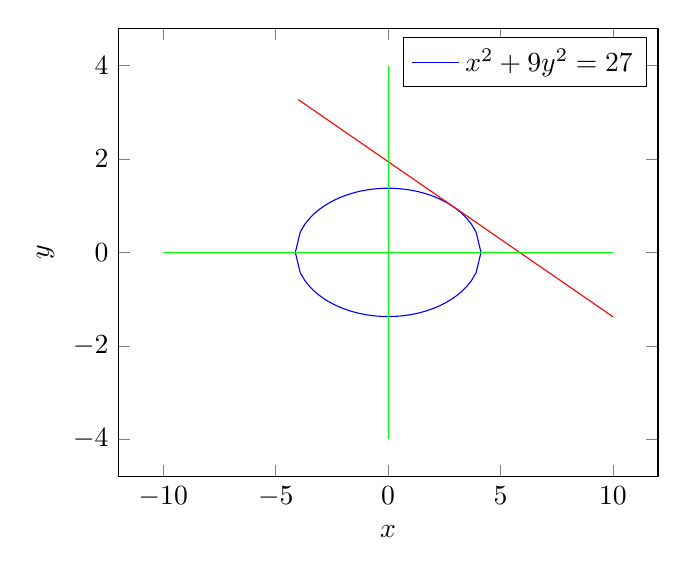
\begin{tikzpicture}
\begin{axis}[
    axis lines = box,
    xlabel = {$x$},
    ylabel = {$y$},
]

%Here the blue parabloa is defined
\addplot [
    domain=-4.123:4.123, 
    samples=40, 
    color=blue,
    ]
    {(17-x^2)^(0.5)/3};
\addplot [
    domain=-4.123:4.123, 
    samples=40, 
    color=blue,
]
{-(17-x^2)^(0.5)/3};    
\addplot[
    domain=-4:10,
    samples =10,
    color=red,
     ]
     {(1.943*(1-x*0.171))};
\addplot[
    domain=-10:10,
    samples=2,
    color=green,
    ]
{0};   
\addplot[
    domain=-0.000000004:0.000000004,
    samples=2,
    color=green,
    ]
{1000000000*x};
\addlegendentry{$x^2+9y^2=27$}
 
\end{axis}
\end{tikzpicture}


                    
\end{frame}
\begin{frame}
    Area of \Delta$OAB$ =(0.5)(\sqrt{17}/\cos\theta)(\sqrt{17}/(3\sin\theta))\\
                    =17/3\sin2\theta\\
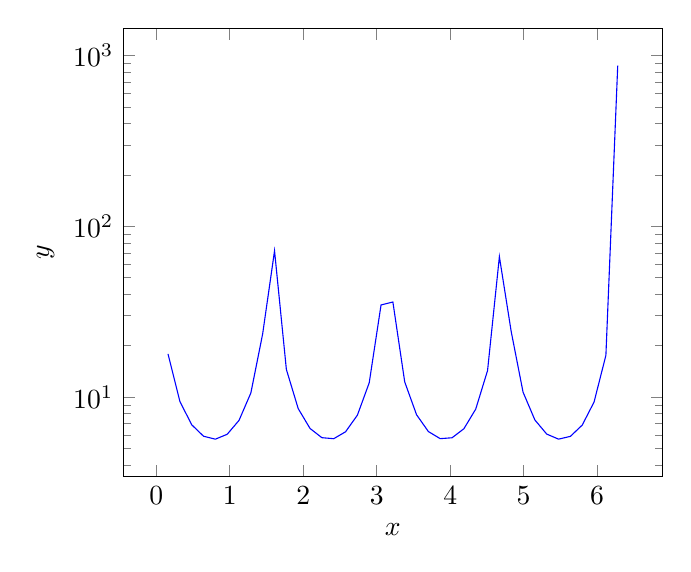
\begin{tikzpicture}
\begin{semilogyaxis}[
    axis lines = box,
    xlabel = {$x$},
    ylabel = {$y$},
]              
\addplot[
    domain=0:6.28, 
    samples=40, 
    color=blue,]
{17/abs(3*sin(deg(2*x))};
\end{semilogyaxis}
\end{tikzpicture}\\
Area has min value when \sin2\theta has max value
\longrightarrow$$
|\sin2\theta|=1
$$

\end{frame}



\end{document}

